\documentclass{article}

\usepackage{fancyvrb}
\usepackage{graphicx}
\usepackage{hyperref}

\graphicspath{ {images/} }

\DefineVerbatimEnvironment{verbatim}{Verbatim}{xleftmargin=.5in}

\author{
  Reinier Maas \\ 4131495
  \and
  Adolfo Ochagavía \\ 4045483
}
\title{CCO - Assignment 2}
\begin{document}

\maketitle

\section{Building and running}

Provided you have \texttt{stack} and \texttt{uuagc} installed on your system, you can use \texttt{make} to build the project.
The project should probably build as well when using \texttt{cabal}, though we haven't tested it.
To also generate the graphs we need \texttt{GraphViz} installed on the system.
Below we explain how to actually run our code.

\subsection*{Analyze a single program}

After compiling the executable, you can run it using the command below:

\begin{verbatim}
stack exec -- mf <max-context-depth> <file>
\end{verbatim}

Here, \texttt{max-context-depth} refers to the maximum length of the context string and \texttt{file} to the path to the file you would like to analyze. For instance, if your working directory is the root of the project, you could try the following\footnote{Note that the code assumes line endings are \texttt{LF}. Since \texttt{git} may change the line endings under the hood, it is possible for the code to have \texttt{CRLF} line endings. If this happens, running the executable will result in an error: \texttt{"argv" (line 1, column 1):unknown parse error}}:

\begin{verbatim}
stack exec -- mf 2 examples/cp1.c
\end{verbatim}

The results of the program are printed as a graph, specified in the DOT language.
Each analysis produces its own graph.
As you may already know, you can use GraphViz to actually get an image of the graph (or you can use \href{http://www.webgraphviz.com/}{this online version}).

Each time you run the program, the Constant Propagation and Strongly Live Variables analysis will be run.
Note that the latter is intraprocedural, so it will not be affected by changes to the \texttt{max-context-depth} parameter.
An excerpt of the output is shown below:

\begin{verbatim}
CP ANALYSIS:
digraph {
// Content replaced by this comment because of its length
}

SLV ANALYSIS:
digraph {
// Content replaced by this comment because of its length
}
\end{verbatim}

\subsection*{Analyze all programs in a given directory}

It is also possible to run the analysis for all programs in a given directory. This can be achieved with the command below:

\begin{verbatim}
stack exec -- mf all <max-context-depth> <inputDir> <outputDir>
\end{verbatim}

Here, \texttt{inputDir} is the path to the directory where the programs are to be found. For instance, you could use \texttt{examples} as a value in order to analyze all files in said directory.

Since the analysis is run for many programs, the output is no longer printed to \texttt{stdout}. Instead, for each program, two files are created which contain the resulting graph after the analysis. Here, the \texttt{.cp} file extension is used to store the results of constant propagation, while the \texttt{.slv} is used to store those of strongly live variables. Naturally, the resulting files are saved in the directory specified through \texttt{outputDir}.

\subsection*{From GHCi}

Running the program from GHCi is almost the same as through the CLI tool. You can do it by calling the \texttt{run} function (e.g. \texttt{run 2 "examples/cp1.c"}) or the \texttt{runAll} function (e.g. \texttt{runAll 2 "examples" "results"}). In fact, the CLI is just a wrapper around the \texttt{run} and \texttt{runAll} functions.

\subsection*{A side-note on the formatting of graphs}

In order to support graphs with more than one entry point and exit points, we add two additional \texttt{skip} nodes; one at the beginning and one at the end. This way we obtain a graph with a single entry point and a single exit point. Since both nodes are \texttt{skip}, they do not have any effect on the results of the analyses.

\section{Implementation details}

% See https://github.com/aochagavia/CompilerConstruction/compare/mf-init...master for a diff

\subsection*{Assumptions}

In order to reduce the complexity of the implementation, we assume that no global variables exist in the programming language.

\subsection*{Modules}

\begin{itemize}
	\item \texttt{Lexer and Parser}: there are no relevant modifications to these modules.
	\item \texttt{Monotone}: implements the \texttt{mfp} function according to the slides of the course. Our implementation supports embellished monotone instances.
	\item \texttt{AttributeGrammar}: see \textbf{Attribute Grammar}.
	\item \texttt{ConstPropagation}: see \textbf{Constant Propagation}.
	\item \texttt{StronglyLiveVariables}: see \textbf{Strongly Live Variables}.
	\item \texttt{Main}: glues everything together in the \texttt{run} function (lexing, parsing, executing the attribute grammar, running the analyses and printing the results).
\end{itemize}

\subsection*{Code samples}

Samples are located in different directories depending on their purpose:

\begin{itemize}
	\item \texttt{examples}: samples to test both analyses.
	\item \texttt{examples/cp}: samples to test constant propagation.
	\item \texttt{examples/slv}: samples to test strongly live variables.
	\item \texttt{examples/error}: samples that should be rejected by our tool.
\end{itemize}

\subsection*{Attribute Grammar}

The starting framework that we used for the assignment came with two definitions of the abstract syntax tree, the second one being just a duplicate of the first, except for the fact that it includes labels for each node. There are mainly two features that we had to implement before we could start working on the analysis part:

\begin{enumerate}
	\item Labeling the AST by transforming the original \texttt{Program} into a \texttt{Program'}.
	\item Building a control flow graph of the resulting \texttt{Program'}. In this step, we included basic support for error detection, such as rejecting programs where \texttt{break} or \texttt{continue} statements appear outside a loop.
\end{enumerate}

\subsection*{MFP implementation}

Our implementation of the MFP algorithm follows the slides and does not require much explanation. Since we support embellished monotone instances, the user needs to provide unary and binary transfer functions. We also provide a \texttt{liftTransfer} function that can be used by monotone instances to lift transfer functions where the context remains unchanged.

\subsection*{Constant Propagation}

The constant propagation analysis is implemented as an embellished monotone instance with support for interprocedural analysis. The value for \texttt{k} is determined by the user through the \texttt{max-context-length} parameter.

The transfer functions are based on the analysis explained during the lectures, with the only difference that we need to account for changes to the context. The unary transfer function is therefore trivially implemented by evaluating the expressions and keeping a map of the values associated to each variable. The binary transfer function, however, is a bit more complex and is used to handle edges starting at procedures (\texttt{Proc'}) or calls (\texttt{Call'}).

The transfer function when the edge starts at the entry of a \texttt{Proc'} is the identity function. However, when the edge starts at the exit of a \texttt{Proc}, things get more complicated, since we need to combine the results of the analysis of the procedure with the information we have at the call site. This happens in the \texttt{transferProc} function.

The transfer function when the edge involves a \texttt{Call'} considers three cases:

\begin{enumerate}
	\item The edge goes from call entry to call exit (at the call site): joins the analysis from the procedure with the current analysis.
	\item The edge goes from call entry to procedure start: pushes a new label to the call string and translates the argument expressions to the parameter names.
	\item The edge goes from call exit to something else: applies the identity function.
\end{enumerate}

In the lattice, each variable is mapped to one of the following items:

% Stolen from https://cseweb.ucsd.edu/classes/fa03/cse231/lec10seq.pdf
\begin{enumerate}
	\item $\top$, meaning that the variable may be a constant but our analysis cannot prove it;
	\item $\bot$, meaning that the variable is undefined;
	\item $k$ (a boolean or integral value), meaning that the variable has the constant value of $k$;
\end{enumerate}

The operations on the lattice are defined by pattern matching as follows:

\begin{itemize}
	\item $x \sqcup \top = \top$
	\item $x \sqcup \bot = x$
	\item $x \sqcup y = \mathbf{if}\ x == y\ \mathbf{then}\ x\ \mathbf{else}\ \top$
	\item $x \sqsubseteq y = x == y$
\end{itemize}

\subsection*{Strongly Live Variables}

The strongly live variables analysis is implemented as an embellished monotone instance, but it only supports intraprocedural analysis. This means that the \texttt{max-content-length} parameter is ignored and the value of \texttt{k} is always zero.

Regarding the transfer functions, the binary transfer function just ignores the second parameter and calls the unary transfer function under the hood. The implementation of the unary transfer function is based on gen sets and kill sets, as explained during the lecture.

In this analysis we follow the approach in the book, which means that the we assume no variables will be used at the end of the program.

As explained in the lectures, the lattice is defined as:

\begin{itemize}
	\item $L = \mathcal{P}(\mathbf{Var_*})$ (finite sets of variables)
	\item $\sqcup\ =\ \cup$ and $\sqsubseteq\ =\ \subseteq$
	\item $\bot = \emptyset$ and $\top = \mathbf{Var_*}$
\end{itemize}

\section{Analyses walkthrough}

\subsection*{Constant Propagation}

To showcase constant propagation, we walk through the analysis of the \texttt{easy.c} program in \texttt{examples/cp}. The results of the analysis can be observed in Figure \ref{fig-cp} and are explained below. While we would have preferred to walk through a more complex case, it would result in a much bigger graph and would be impossible to include in a sensible way in this document.

First of all, notice that there are two \texttt{skip} nodes that do not appear in the original program. those are inserted by our tool at the beginning and at the end of the graph. Since they do not have any influence in the output of the analysis we are going to ignore them.

At node 0, we see that the initial list of available constants is empty, which is another way to indicate that the value associated to each variable is $\top$. However, at the end of said node we see that the constant value associated to $x$ has changed and is now 42. This result propagates to node 1 and after processing the statement we know the value of $y$ as well. The situation with node 2 is analogous. Node 3 redefines the value of $x$ and you can see that it is correctly updated in the list of available constants.

\begin{figure}
\centering
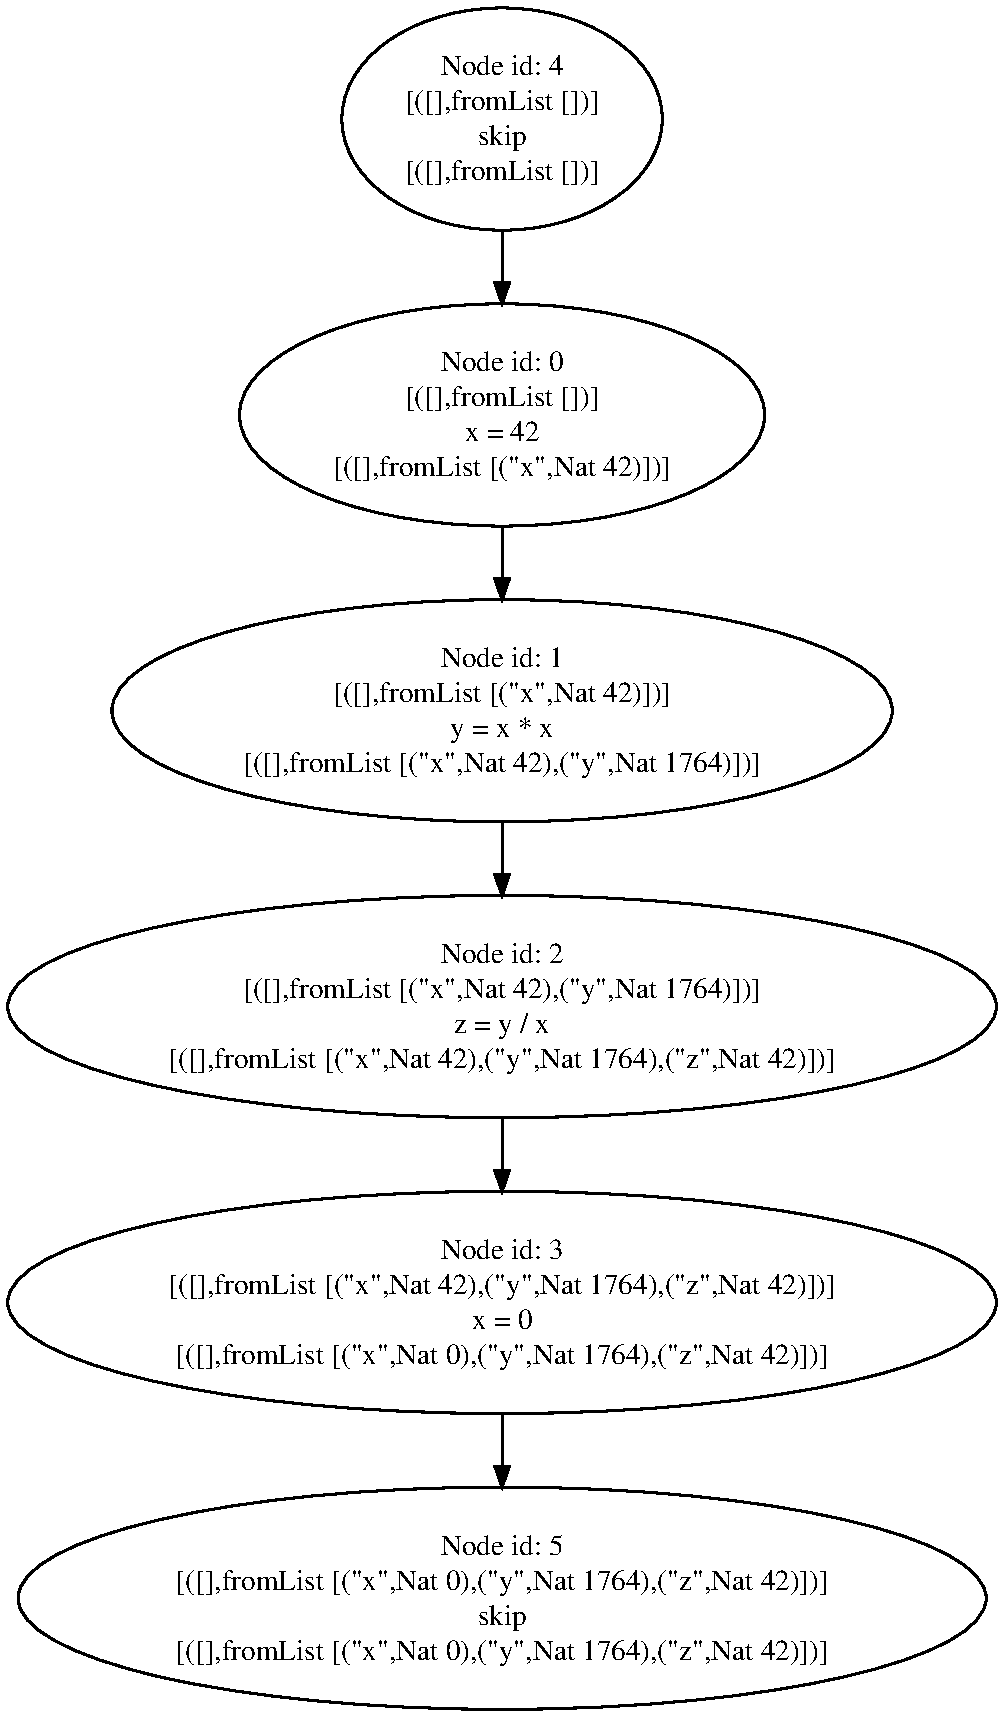
\includegraphics[width=11cm, height=18cm]{cp_easy}
\caption{Constant propagation analysis for the \texttt{easy\_cp.c} program.}
\label{fig-cp}
\end{figure}

\subsection*{Strongly Live Variables}

To showcase strongly live variables propagation, we walk through the analysis of the \texttt{ifthenelse1.c} program in \texttt{examples/slv}. The results of the analysis can be observed in Figure \ref{fig-slv} and are explained below.

As expected, node 0 shows that there are no live variables live at the beginning of the program. However, $x$ becomes live after the assignment, since it is going to be used by node 2. The analysis propagates this information backwards through the graph. Our analysis is not smart enough to know that the true branch will always be taken, so $x$ would be live even if it was only used by node 3. However, you can see that $x$ is no longer live at the beginning of node 3, while it does live at the beginning of node 2.

Finally, as you can observe from looking at node 6, there are no live variables at the end of the program. This is consistent with our choice of following the approach used in the book, where it is assumed that no variables are read after the program ends.

\begin{figure}
	\centering
	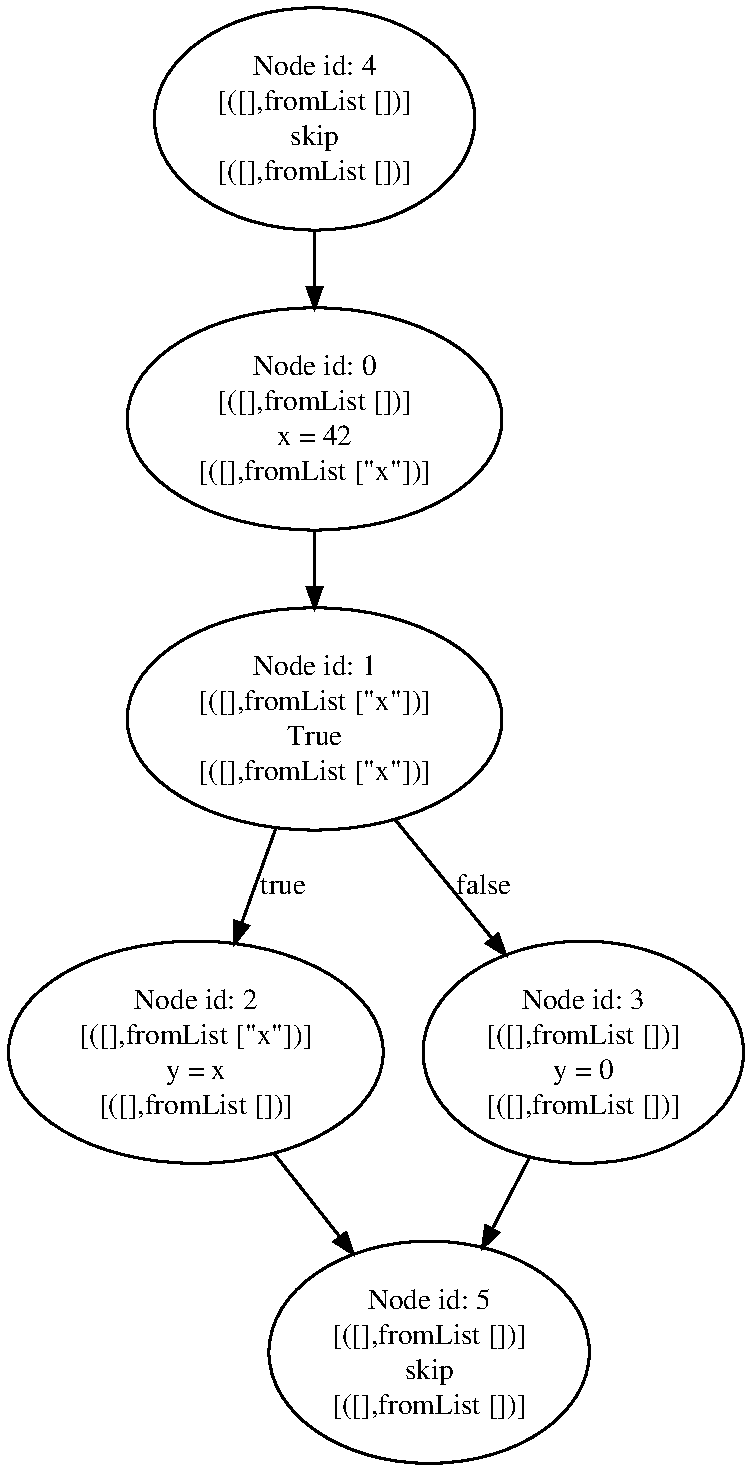
\includegraphics[width=9cm, height=18cm]{slv_ifthenelse1}
	\caption{Strongly live variable analysis for the \texttt{ifthenelse1.c} program.}
	\label{fig-slv}
\end{figure}

\end{document}
